%%%%%%%%%%%%%%%%%%%%%%%%%%%%%%%%%%%%%%%%%%%%%%%%%%%%%%%%%%%%%%%
%
% Welcome to Overleaf --- just edit your article on the left,
% and we'll compile it for you on the right. If you give
% someone the link to this page, they can edit at the same
% time. See the help menu above for more info. Enjoy!
%
%%%%%%%%%%%%%%%%%%%%%%%%%%%%%%%%%%%%%%%%%%%%%%%%%%%%%%%%%%%%%%%
%
% For more detailed article preparation guidelines, please see:
% https://f1000research.com/for-authors/article-guidelines/software-tool-articles and http://f1000research.com/data-preparation

\documentclass[9pt,a4paper]{extarticle}
\usepackage{f1000_styles}

%% Default: numerical citations
\usepackage[numbers]{natbib}

%% Uncomment this lines for superscript citations instead
% \usepackage[super]{natbib}

%% Uncomment these lines for author-year citations instead
% \usepackage[round]{natbib}
% \let\cite\citep

%% syntax highlighting style kate
\renewcommand{\KeywordTok}[1]{\textbf{{#1}}}
\renewcommand{\DataTypeTok}[1]{\textcolor[rgb]{0.50,0.00,0.00}{{#1}}}
\renewcommand{\DecValTok}[1]{\textcolor[rgb]{0.00,0.00,1.00}{{#1}}}
\renewcommand{\BaseNTok}[1]{\textcolor[rgb]{0.00,0.00,1.00}{{#1}}}
\renewcommand{\FloatTok}[1]{\textcolor[rgb]{0.50,0.00,0.50}{{#1}}}
\renewcommand{\ConstantTok}[1]{\textcolor[rgb]{0.00,0.00,0.00}{{#1}}}
\renewcommand{\CharTok}[1]{\textcolor[rgb]{1.00,0.00,1.00}{{#1}}}
\renewcommand{\SpecialCharTok}[1]{\textcolor[rgb]{1.00,0.00,1.00}{{#1}}}
\renewcommand{\StringTok}[1]{\textcolor[rgb]{0.87,0.00,0.00}{{#1}}}
\renewcommand{\VerbatimStringTok}[1]{\textcolor[rgb]{0.87,0.00,0.00}{{#1}}}
\renewcommand{\SpecialStringTok}[1]{\textcolor[rgb]{0.87,0.00,0.00}{{#1}}}
\renewcommand{\ImportTok}[1]{{#1}}
\renewcommand{\CommentTok}[1]{\textcolor[rgb]{0.50,0.50,0.50}{\textit{{#1}}}}
\renewcommand{\DocumentationTok}[1]{\textcolor[rgb]{0.50,0.50,0.50}{\textit{{#1}}}}
\renewcommand{\AnnotationTok}[1]{\textcolor[rgb]{0.50,0.50,0.50}{\textbf{\textit{{#1}}}}}
\renewcommand{\CommentVarTok}[1]{\textcolor[rgb]{0.50,0.50,0.50}{\textbf{\textit{{#1}}}}}
\renewcommand{\OtherTok}[1]{{#1}}
\renewcommand{\FunctionTok}[1]{\textcolor[rgb]{0.00,0.00,0.50}{{#1}}}
\renewcommand{\VariableTok}[1]{{#1}}
\renewcommand{\ControlFlowTok}[1]{{#1}}
\renewcommand{\OperatorTok}[1]{{#1}}
\renewcommand{\BuiltInTok}[1]{{#1}}
\renewcommand{\ExtensionTok}[1]{{#1}}
\renewcommand{\PreprocessorTok}[1]{\textbf{{#1}}}
\renewcommand{\AttributeTok}[1]{{#1}}
\renewcommand{\RegionMarkerTok}[1]{{#1}}
\renewcommand{\InformationTok}[1]{\textcolor[rgb]{0.50,0.50,0.50}{\textbf{\textit{{#1}}}}}
\renewcommand{\WarningTok}[1]{\textcolor[rgb]{1.00,0.00,0.00}{\textbf{{#1}}}}
\renewcommand{\AlertTok}[1]{\textcolor[rgb]{0.00,1.00,0.00}{\textbf{{#1}}}}
\renewcommand{\ErrorTok}[1]{\textcolor[rgb]{1.00,0.00,0.00}{\textbf{{#1}}}}
\renewcommand{\NormalTok}[1]{{#1}}

\begin{document}
\pagestyle{front}

\title{valr: Reproducible genome interval analysis in R}
\author[1]{Kent A. Riemondy}
\author[1]{Austin Gillen}
\author[2]{Ryan M. Sheridan}
\author[2]{Yinni Yu}
\author[3]{Christopher G. Bennett}
\author[1,2,*]{Jay R. Hesselberth}

\affil[1]{University of Colorado School of Medicine, RNA Bioscience Initiative, Aurora CO 80045}
\affil[2]{University of Colorado School of Medicine, Department of Biochemistry and Molecular Genetics}
\affil[3]{ComAnalyzeIT LLC, Fort Collins CO 80525}
\affil[*]{Corresponding author: jay.hesselberth@gmail.com}

\maketitle
\thispagestyle{front}

% 300 words
\begin{abstract}
New tools for reproducible exploratory data analysis of large data sets are important to address the rising size and complexity of genomic data. We developed the \texttt{valr} R package to enable flexible and efficient genomic interval analysis. \texttt{valr} leverages new tools available in the "tidyverse" including \texttt{dplyr}. Benchmarks of \texttt{valr} show it performs similar to \texttt{BEDtools} and can be used for interactive  analyses and incorporated into existing analysis pipelines.

\end{abstract}

\section*{Keywords}

Genomics, Intervals, BEDtools, reproducibility, R, RStudio

\clearpage
\pagestyle{main}
\section*{Introduction}

	A routine bioinformatic task is the analysis of the relationships between sets of genomic intervals including the identification of DNA variants within genetic regions, annotation of regions enriched for nucleic acid binding proteins, and computation of read density within a set of exons. Command-line tools for interval analysis such as BEDtools \cite{quinlan_bedtools:_2010} and BEDOPS \cite{neph_bedops:_2012} enable analyses of genome-wide datasets and are keys components of analysis pipelines. Analyses with these tools commonly combine processing intervals on the command-line with visualization and statistical analysis in R. However, the need to master both the command-line and R hinders exploratory data analysis, and the development reproducible research workflows built in the RMarkdown framework.

	Existing R packages developed for interval analysis include IRanges \cite{lawrence_software_2013}, bedr \cite{haider_bedr_2016}, and GenometriCorr \cite{favorov_exploring_2012}. IRanges is a Bioconductor package that provides  interval classes and methods to perform interval arithmetic and is used by many Bioconductor packages. bedr is a CRAN-distributed package that provides wrapper R functions to call the BEDTools, BedOPS, and tabix command-line utilities, providing out-of-memory support for interval analysis. Finally,  GenometriCorr provides a set of statistical tests to determine the relationships between interval sets using IRanges data structures. These packages provide  functionality for processing and statistical inference of interval data, but they do not easily integrate with interactive data visualization features developed for R including Shiny\cite{chang_shiny_2017}, and the RStudio IDE. Moreover, the S4 data structures implemented by IRanges do not easily interface with the recent advances provided by the popular tidyverse suite of data processing and visualization tools (e.g., dplyr, purrr, broom, and ggplot2) \cite{wickham_tidyverse_2017}. We sought to develop an flexible R package for genomic interval arithmetic built to incorporate new R programming, visualization, and interactivity features.

\section*{Methods}

\subsection*{Implementation}
valr is an R package that makes extensive use of dplyr, a flexible and high-performance framework for data manipulation in R \cite{wickham_dplyr_2016}. Compute intensive functions in valr are written in C++ using Rcpp to enable fluid interactive analysis of large datasets\cite{eddelbuettel_rcpp_2011}. Interval intersections and related operations use an interval tree algorithm to efficiently search for overlapping intervals\cite{cormen_2001}. BED files are imported and handled in R as data\_frame objects, requiring minimal pre or post-processing to integrate with additional R packages or command line tools.

\subsection*{Operation}
valr is distributed as part of the CRAN R package repository and is compatible with Mac OS X, Windows, and major Linux operating systems. Package dependencies and system requirements are documented in the valr CRAN repository (\url{https://cran.r-project.org/web/packages/valr/index.html}).

\section*{Use Cases}
To demonstrate the functionality and utility of \texttt{valr}, presented below is a basic tutorial for using valr and additional common use cases for genomic interval analysis.

\subsection*{Basic Usage}

\subsubsection*{Input data}\label{input-data}

\texttt{valr} provides a set of functions to read BED, BEDgraph, and VCF formats into R as convenient \texttt{tibble} data\_frame objects. All tbls have \texttt{chrom}, \texttt{start}, and \texttt{end} columns, and tbls from multi-column formats have additional pre-determined column names. Standards methods for importing data (e.g. \texttt{read.table}, \texttt{readr::read\_tsv}) are also supported provided the constructed dataframes contain the requisite column names (\texttt{chrom}, \texttt{start}, \texttt{end}). Additionally \texttt{valr} supports connections to remote databases to programatically access the UCSC and Ensembl databases via the \texttt{db\_ucsc} and \texttt{db\_ensembl} functions.

\begin{Highlighting}[]
\KeywordTok{library}\NormalTok{(valr)}
\CommentTok{# function to retrieve path to example data}
\NormalTok{bed_filepath <-}\StringTok{ }\KeywordTok{valr_example}\NormalTok{(}\StringTok{"3fields.bed.gz"}\NormalTok{) }
\KeywordTok{read_bed}\NormalTok{(bed_filepath) }
\CommentTok{#> # A tibble: 10 x 3}
\CommentTok{#>    chrom  start    end}
\CommentTok{#>    <chr>  <int>  <int>}
\CommentTok{#>  1  chr1  11873  14409}
\CommentTok{#>  2  chr1  14361  19759}
\CommentTok{#>  3  chr1  14406  29370}
\CommentTok{#>  4  chr1  34610  36081}
\CommentTok{#>  5  chr1  69090  70008}
\CommentTok{#>  6  chr1 134772 140566}
\CommentTok{#>  7  chr1 321083 321115}
\CommentTok{#>  8  chr1 321145 321207}
\CommentTok{#>  9  chr1 322036 326938}
\CommentTok{#> 10  chr1 327545 328439}

\CommentTok{#using URL}
\KeywordTok{read_bed}\NormalTok{(}\StringTok{"https://github.com/rnabioco/valr/raw/master/inst/extdata/3fields.bed.gz"}\NormalTok{)}
\CommentTok{#> # A tibble: 10 x 3}
\CommentTok{#>    chrom  start    end}
\CommentTok{#>    <chr>  <int>  <int>}
\CommentTok{#>  1  chr1  11873  14409}
\CommentTok{#>  2  chr1  14361  19759}
\CommentTok{#>  3  chr1  14406  29370}
\CommentTok{#>  4  chr1  34610  36081}
\CommentTok{#>  5  chr1  69090  70008}
\CommentTok{#>  6  chr1 134772 140566}
\CommentTok{#>  7  chr1 321083 321115}
\CommentTok{#>  8  chr1 321145 321207}
\CommentTok{#>  9  chr1 322036 326938}
\CommentTok{#> 10  chr1 327545 328439}
\end{Highlighting}


\subsubsection*{Example of combining valr tools}

The functions in \texttt{valr} have similar names to their \texttt{BEDtools} counterparts, and so will be familiar to users of the \texttt{BEDtools} suite. Also, similar to pybedtools\cite{dale_pybedtools:_2011}, a python wrapper for \texttt{BEDTools}, \texttt{valr} has a terse syntax. For example, shown below is a demonstration of how to find all intergenic SNPs within 1 kilobase of genes using \texttt{valr}.

\begin{Highlighting}[]
\KeywordTok{library}\NormalTok{(dplyr)}

\NormalTok{snps <-}\StringTok{ }\KeywordTok{read_bed}\NormalTok{(}\KeywordTok{valr_example}\NormalTok{(}\StringTok{'hg19.snps147.chr22.bed.gz'}\NormalTok{), }\DataTypeTok{n_fields =} \DecValTok{6}\NormalTok{)}
\NormalTok{genes <-}\StringTok{ }\KeywordTok{read_bed}\NormalTok{(}\KeywordTok{valr_example}\NormalTok{(}\StringTok{'genes.hg19.chr22.bed.gz'}\NormalTok{), }\DataTypeTok{n_fields =} \DecValTok{6}\NormalTok{)}

\CommentTok{# find snps in intergenic regions}
\NormalTok{intergenic <-}\StringTok{ }\KeywordTok{bed_subtract}\NormalTok{(snps, genes)}
\CommentTok{# distance from intergenic snps to nearest gene}
\NormalTok{nearby <-}\StringTok{ }\KeywordTok{bed_closest}\NormalTok{(intergenic, genes)}

\NormalTok{nearby %>%}
\StringTok{  }\KeywordTok{select}\NormalTok{(}\KeywordTok{starts_with}\NormalTok{(}\StringTok{'name'}\NormalTok{), .overlap, .dist) %>%}
\StringTok{  }\KeywordTok{filter}\NormalTok{(}\KeywordTok{abs}\NormalTok{(.dist) <}\StringTok{ }\DecValTok{1000}\NormalTok{)}
\CommentTok{#> # A tibble: 285 x 4}
\CommentTok{#>         name.x            name.y .overlap .dist}
\CommentTok{#>          <chr>             <chr>    <int> <int>}
\CommentTok{#>  1   rs2261631             P704P        0  -267}
\CommentTok{#>  2 rs570770556             POTEH        0  -912}
\CommentTok{#>  3 rs538163832             POTEH        0  -952}
\CommentTok{#>  4   rs9606135            TPTEP1        0  -421}
\CommentTok{#>  5  rs11912392 ANKRD62P1-PARP4P3        0   104}
\CommentTok{#>  6   rs8136454          BC038197        0   355}
\CommentTok{#>  7   rs5992556              XKR3        0  -455}
\CommentTok{#>  8 rs114101676              GAB4        0   473}
\CommentTok{#>  9  rs62236167             CECR7        0   261}
\CommentTok{#> 10   rs5747023             CECR1        0  -386}
\CommentTok{#> # ... with 275 more rows}
\end{Highlighting}

\subsubsection*{Visual documentation}\label{visual-documentation}
By conducting interval arithmetic entirely in R, \texttt{valr} is also an effective teaching tool for introducing interval analysis to early-stage analysts without requiring familiarity with both command-line tools and R. To aid in demonstrating the interval operations available in \texttt{valr}, we developed the \texttt{bed\_glyph()} tool which produces plots demonstrating the input and output of operations in \texttt{valr} in a manner similar to those found in the \texttt{BEDtools} documentation.
Shown below is the code required to produce glyphs displaying the results of intersecting \texttt{x} and \texttt{y} intervals with \texttt{bed\_intersect()} , and the result of merging \texttt{x} intervals with \texttt{bed\_merge()} (Figure 1 \ref{fig:Figure 1}).

\begin{Highlighting}[]
\NormalTok{x <-}\StringTok{ }\NormalTok{tibble::}\KeywordTok{tribble}\NormalTok{(}
  \NormalTok{~chrom, ~start, ~end,}
  \StringTok{'chr1'}\NormalTok{, }\DecValTok{25}\NormalTok{,     }\DecValTok{50}\NormalTok{,}
  \StringTok{'chr1'}\NormalTok{, }\DecValTok{100}\NormalTok{,    }\DecValTok{125}
\NormalTok{)}

\NormalTok{y <-}\StringTok{ }\NormalTok{tibble::}\KeywordTok{tribble}\NormalTok{(}
  \NormalTok{~chrom, ~start, ~end,}
  \StringTok{'chr1'}\NormalTok{, }\DecValTok{30}\NormalTok{,     }\DecValTok{75}
\NormalTok{)}

\KeywordTok{bed_glyph}\NormalTok{(}\KeywordTok{bed_intersect}\NormalTok{(x, y))}
\end{Highlighting}

And this glyph illustrates \texttt{bed\_merge()}:

\begin{Highlighting}[]
\NormalTok{x <-}\StringTok{ }\NormalTok{tibble::}\KeywordTok{tribble}\NormalTok{(}
  \NormalTok{~chrom, ~start, ~end,}
  \StringTok{'chr1'}\NormalTok{,      }\DecValTok{1}\NormalTok{,      }\DecValTok{50}\NormalTok{,}
  \StringTok{'chr1'}\NormalTok{,      }\DecValTok{10}\NormalTok{,     }\DecValTok{75}\NormalTok{,}
  \StringTok{'chr1'}\NormalTok{,      }\DecValTok{100}\NormalTok{,    }\DecValTok{120}
\NormalTok{)}

\KeywordTok{bed_glyph}\NormalTok{(}\KeywordTok{bed_merge}\NormalTok{(x))}
\end{Highlighting}
% * <jay.hesselberth@gmail.com> 2017-06-10T17:17:56.304Z:
%
% Is it possible to insert the figure inline in the document?
% * KR
% Yes, but they request that figures are listed at the end of the document.
% Once the document is formatted by F1000 I think that the document will look similar to this article:
% https://f1000research.com/articles/5-2122/v2
% ^.


\subsubsection*{Grouping data}\label{grouping-data}

The \texttt{group\_by} function in dplyr can be used to perform functions
on subsets of single and multiple \texttt{data\_frame}s. Functions in
\texttt{valr} leverage grouping to enable a variety of comparisons. For
example, intervals can be grouped by \texttt{strand} to perform
comparisons among intervals on the same strand.

\begin{Highlighting}[]
\NormalTok{x <-}\StringTok{ }\NormalTok{tibble::}\KeywordTok{tribble}\NormalTok{(}
  \NormalTok{~chrom, ~start, ~end, ~strand,}
  \StringTok{'chr1'}\NormalTok{, }\DecValTok{1}\NormalTok{,      }\DecValTok{100}\NormalTok{,  }\StringTok{'+'}\NormalTok{,}
  \StringTok{'chr1'}\NormalTok{, }\DecValTok{50}\NormalTok{,     }\DecValTok{150}\NormalTok{,  }\StringTok{'+'}\NormalTok{,}
  \StringTok{'chr2'}\NormalTok{, }\DecValTok{100}\NormalTok{,    }\DecValTok{200}\NormalTok{,  }\StringTok{'-'}
\NormalTok{)}

\NormalTok{y <-}\StringTok{ }\NormalTok{tibble::}\KeywordTok{tribble}\NormalTok{(}
  \NormalTok{~chrom, ~start, ~end, ~strand,}
  \StringTok{'chr1'}\NormalTok{, }\DecValTok{50}\NormalTok{,     }\DecValTok{125}\NormalTok{,  }\StringTok{'+'}\NormalTok{,}
  \StringTok{'chr1'}\NormalTok{, }\DecValTok{50}\NormalTok{,     }\DecValTok{150}\NormalTok{,  }\StringTok{'-'}\NormalTok{,}
  \StringTok{'chr2'}\NormalTok{, }\DecValTok{50}\NormalTok{,     }\DecValTok{150}\NormalTok{,  }\StringTok{'+'}
\NormalTok{)}

\CommentTok{# intersect tbls by strand}
\NormalTok{x <-}\StringTok{ }\KeywordTok{group_by}\NormalTok{(x, strand)}
\NormalTok{y <-}\StringTok{ }\KeywordTok{group_by}\NormalTok{(y, strand)}

\KeywordTok{bed_intersect}\NormalTok{(x, y)}
\CommentTok{#> # A tibble: 2 x 8}
\CommentTok{#>   chrom start.x end.x strand.x start.y end.y strand.y .overlap}
\CommentTok{#>   <chr>   <dbl> <dbl>    <chr>   <dbl> <dbl>    <chr>    <int>}
\CommentTok{#> 1  chr1       1   100        +      50   125        +       50}
\CommentTok{#> 2  chr1      50   150        +      50   125        +       75}
\end{Highlighting}

Comparisons between intervals on opposite strands are done using the
\texttt{flip\_strands()} function:

\begin{Highlighting}[]
\NormalTok{x <-}\StringTok{ }\KeywordTok{group_by}\NormalTok{(x, strand)}

\NormalTok{y <-}\StringTok{ }\KeywordTok{flip_strands}\NormalTok{(y)}
\NormalTok{y <-}\StringTok{ }\KeywordTok{group_by}\NormalTok{(y, strand)}

\KeywordTok{bed_intersect}\NormalTok{(x, y)}
\CommentTok{#> # A tibble: 3 x 8}
\CommentTok{#>   chrom start.x end.x strand.x start.y end.y strand.y .overlap}
\CommentTok{#>   <chr>   <dbl> <dbl>    <chr>   <dbl> <dbl>    <chr>    <int>}
\CommentTok{#> 1  chr2     100   200        -      50   150        -       50}
\CommentTok{#> 2  chr1       1   100        +      50   150        +       50}
\CommentTok{#> 3  chr1      50   150        +      50   150        +      100}
\end{Highlighting}

Both single set (e.g. \texttt{bed\_merge()}) and multi set operations
will respect groupings in the input intervals.

\subsubsection*{Column specification}\label{column-specification}

Columns in \texttt{BEDtools} are referred to by position:

\begin{Highlighting}[]
\CommentTok{# calculate the mean of column 6 for intervals in `b` that overlap with `a`}
\KeywordTok{bedtools} \NormalTok{map -a a.bed -b b.bed -c 6 -o mean}
\end{Highlighting}

In \texttt{valr}, columns are referred to by name and can be used in
multiple name/value expressions for summaries.

\begin{Highlighting}[]
\CommentTok{# calculate the mean and variance for a `value` column}
\KeywordTok{bed_map}\NormalTok{(a, b, }\DataTypeTok{.mean =} \KeywordTok{mean}\NormalTok{(value), }\DataTypeTok{.var =} \KeywordTok{var}\NormalTok{(value))}

\CommentTok{# report concatenated and max values for merged intervals}
\KeywordTok{bed_merge}\NormalTok{(a, }\DataTypeTok{.concat =} \KeywordTok{concat}\NormalTok{(value), }\DataTypeTok{.max =} \KeywordTok{max}\NormalTok{(value))}
\end{Highlighting}


\subsubsection*{API}\label{api}
The major functions available in valr are shown in Table \ref{tab:tools}.


\subsection*{Summarizing interval coverage across genomic features}

This demonstration illustrates how to use \texttt{valr} tools to perform
a ``meta-analysis'' of signals relative to genomic features. Here we
analyze the distribution of histone marks surrounding transcription
start sites, using H3K4Me3 Chip-Seq data downloaded from ENCODE.

First we load packages and relevant data.

\begin{Highlighting}[]
\CommentTok{# `valr_example()` identifies the path of example files in the valr package}
\NormalTok{bedfile <-}\StringTok{ }\KeywordTok{valr_example}\NormalTok{(}\StringTok{'genes.hg19.chr22.bed.gz'}\NormalTok{)}
\NormalTok{genomefile <-}\StringTok{ }\KeywordTok{valr_example}\NormalTok{(}\StringTok{'hg19.chrom.sizes.gz'}\NormalTok{)}
\NormalTok{bgfile  <-}\StringTok{ }\KeywordTok{valr_example}\NormalTok{(}\StringTok{'hela.h3k4.chip.bg.gz'}\NormalTok{)}

\NormalTok{genes <-}\StringTok{ }\KeywordTok{read_bed}\NormalTok{(bedfile, }\DataTypeTok{n_fields =} \DecValTok{6}\NormalTok{)}
\NormalTok{genome <-}\StringTok{ }\KeywordTok{read_genome}\NormalTok{(genomefile)}
\NormalTok{y <-}\StringTok{ }\KeywordTok{read_bedgraph}\NormalTok{(bgfile)}
\end{Highlighting}

Then we generate 1 bp intervals to represent transcription start sites
(TSSs). We focus on \texttt{+} strand genes, but \texttt{-} genes are
easily accommodated by filtering them and using
\texttt{bed\_makewindows()} with \texttt{reversed} window numbers.

\begin{Highlighting}[]
\CommentTok{# generate 1 bp TSS intervals, `+` strand only}
\NormalTok{tss <-}\StringTok{ }\NormalTok{genes %>%}
\StringTok{  }\KeywordTok{filter}\NormalTok{(strand ==}\StringTok{ '+'}\NormalTok{) %>%}
\StringTok{  }\KeywordTok{mutate}\NormalTok{(}\DataTypeTok{end =} \NormalTok{start +}\StringTok{ }\DecValTok{1}\NormalTok{)}

\CommentTok{# 1000 bp up and downstream}
\NormalTok{region_size <-}\StringTok{ }\DecValTok{1000}
\CommentTok{# 50 bp windows}
\NormalTok{win_size <-}\StringTok{ }\DecValTok{50}

\CommentTok{# add slop to the TSS, break into windows and add a group}
\NormalTok{x <-}\StringTok{ }\NormalTok{tss %>%}
\StringTok{  }\KeywordTok{bed_slop}\NormalTok{(genome, }\DataTypeTok{both =} \NormalTok{region_size) %>%}
\StringTok{  }\KeywordTok{bed_makewindows}\NormalTok{(genome, win_size)}

\NormalTok{x}
\CommentTok{#> # A tibble: 13,530 x 7}
\CommentTok{#>    chrom    start      end      name score strand .win_id}
\CommentTok{#>    <chr>    <int>    <int>     <chr> <chr>  <chr>   <int>}
\CommentTok{#>  1 chr22 16161065 16161115 LINC00516     3      +       1}
\CommentTok{#>  2 chr22 16161115 16161165 LINC00516     3      +       2}
\CommentTok{#>  3 chr22 16161165 16161215 LINC00516     3      +       3}
\CommentTok{#>  4 chr22 16161215 16161265 LINC00516     3      +       4}
\CommentTok{#>  5 chr22 16161265 16161315 LINC00516     3      +       5}
\CommentTok{#>  6 chr22 16161315 16161365 LINC00516     3      +       6}
\CommentTok{#>  7 chr22 16161365 16161415 LINC00516     3      +       7}
\CommentTok{#>  8 chr22 16161415 16161465 LINC00516     3      +       8}
\CommentTok{#>  9 chr22 16161465 16161515 LINC00516     3      +       9}
\CommentTok{#> 10 chr22 16161515 16161565 LINC00516     3      +      10}
\CommentTok{#> # ... with 13,520 more rows}
\end{Highlighting}

Now we use the \texttt{.win\_id} group with \texttt{bed\_map()} to
calculate a sum by mapping \texttt{y} signals onto the intervals in
\texttt{x}. These data are regrouped by \texttt{.win\_id} and a summary
with \texttt{mean} and \texttt{sd} values is calculated.

\begin{Highlighting}[]
\CommentTok{# map signals to TSS regions and calculate summary statistics.}
\NormalTok{res <-}\StringTok{ }\KeywordTok{bed_map}\NormalTok{(x, y, }\DataTypeTok{win_sum =} \KeywordTok{sum}\NormalTok{(value, }\DataTypeTok{na.rm =} \OtherTok{TRUE}\NormalTok{)) %>%}
\StringTok{  }\KeywordTok{group_by}\NormalTok{(.win_id) %>%}
\StringTok{  }\KeywordTok{summarize}\NormalTok{(}\DataTypeTok{win_mean =} \KeywordTok{mean}\NormalTok{(win_sum, }\DataTypeTok{na.rm =} \OtherTok{TRUE}\NormalTok{),}
            \DataTypeTok{win_sd =} \KeywordTok{sd}\NormalTok{(win_sum, }\DataTypeTok{na.rm =} \OtherTok{TRUE}\NormalTok{))}

\NormalTok{res}
\CommentTok{#> # A tibble: 41 x 3}
\CommentTok{#>    .win_id win_mean    win_sd}
\CommentTok{#>      <int>    <dbl>     <dbl>}
\CommentTok{#>  1       1 100.8974  85.83423}
\CommentTok{#>  2       2 110.6829  81.13521}
\CommentTok{#>  3       3 122.9070  99.09635}
\CommentTok{#>  4       4 116.2800  96.30098}
\CommentTok{#>  5       5 116.3500 102.33773}
\CommentTok{#>  6       6 124.9048  95.08887}
\CommentTok{#>  7       7 122.9437  94.39792}
\CommentTok{#>  8       8 127.5946  91.47407}
\CommentTok{#>  9       9 130.2051  95.71309}
\CommentTok{#> 10      10 130.1220  88.82809}
\CommentTok{#> # ... with 31 more rows}
\end{Highlighting}

Finally, these summary statistics are used to construct a plot that
illustrates histone density surrounding TSSs (Figure 2\ref{fig:Figure 2}).

\begin{Highlighting}[]
\KeywordTok{library}\NormalTok{(ggplot2)}

\NormalTok{x_labels <-}\StringTok{ }\KeywordTok{seq}\NormalTok{(-region_size, region_size, }\DataTypeTok{by =} \NormalTok{win_size *}\StringTok{ }\DecValTok{5}\NormalTok{)}
\NormalTok{x_breaks <-}\StringTok{ }\KeywordTok{seq}\NormalTok{(}\DecValTok{1}\NormalTok{, }\DecValTok{41}\NormalTok{, }\DataTypeTok{by =} \DecValTok{5}\NormalTok{)}

\NormalTok{sd_limits <-}\StringTok{ }\KeywordTok{aes}\NormalTok{(}\DataTypeTok{ymax =} \NormalTok{win_mean +}\StringTok{ }\NormalTok{win_sd, }\DataTypeTok{ymin =} \NormalTok{win_mean -}\StringTok{ }\NormalTok{win_sd)}

\KeywordTok{ggplot}\NormalTok{(res, }\KeywordTok{aes}\NormalTok{(}\DataTypeTok{x =} \NormalTok{.win_id, }\DataTypeTok{y =} \NormalTok{win_mean)) +}
\StringTok{  }\KeywordTok{geom_point}\NormalTok{() +}\StringTok{ }\KeywordTok{geom_pointrange}\NormalTok{(sd_limits) +}\StringTok{ }
\StringTok{  }\KeywordTok{scale_x_continuous}\NormalTok{(}\DataTypeTok{labels =} \NormalTok{x_labels, }\DataTypeTok{breaks =} \NormalTok{x_breaks) +}\StringTok{ }
\StringTok{  }\KeywordTok{xlab}\NormalTok{(}\StringTok{'Position (bp from TSS)'}\NormalTok{) +}\StringTok{ }\KeywordTok{ylab}\NormalTok{(}\StringTok{'Signal'}\NormalTok{) +}\StringTok{ }
\StringTok{  }\KeywordTok{ggtitle}\NormalTok{(}\StringTok{'Human H3K4me3 signal near transcription start sites'}\NormalTok{) +}
\StringTok{  }\KeywordTok{theme_classic}\NormalTok{()}
\end{Highlighting}

\subsection*{Interval statistics}\label{interval-statistics}

Estimates of significance for interval overlaps can be obtained by
combining \texttt{bed\_shuffle()}, \texttt{bed\_random()} and the
\texttt{sample\_} functions from \texttt{dplyr} with interval statistics
in \texttt{valr}.

Here we examine the extent of overlap of repeat classes with exons in
the human genome (on \texttt{chr22} only, for simplicity) using the
jaccard similarity index. \texttt{bed\_jaccard()} implements the jaccard
test to examine the similarity between two sets of genomic intervals.
Using \texttt{bed\_shuffle()} and \texttt{replicate()} we generate a
\texttt{data\_frame} containing 100 sets of randomly selected intervals
then calculate the jaccard index for each set against the repeat intervals
to generate a null-distribution of jaccard scores. Finally, an empirical p-value is
calculated from the null-distribution.

\begin{Highlighting}[]
\KeywordTok{library}\NormalTok{(tidyverse, }\DataTypeTok{warn.conflicts =} \NormalTok{F)}

\NormalTok{repeats <-}\StringTok{ }\KeywordTok{read_bed}\NormalTok{(}\KeywordTok{valr_example}\NormalTok{(}\StringTok{'hg19.rmsk.chr22.bed.gz'}\NormalTok{), }\DataTypeTok{n_fields =} \DecValTok{6}\NormalTok{) }
\NormalTok{genome <-}\StringTok{ }\KeywordTok{read_genome}\NormalTok{(}\KeywordTok{valr_example}\NormalTok{(}\StringTok{'hg19.chrom.sizes.gz'}\NormalTok{))}
\NormalTok{genes <-}\StringTok{ }\KeywordTok{read_bed12}\NormalTok{(}\KeywordTok{valr_example}\NormalTok{(}\StringTok{'hg19.refGene.chr22.bed.gz'}\NormalTok{))}
\CommentTok{# convert bed12 to bed with exons}
\NormalTok{exons <-}\StringTok{ }\KeywordTok{bed12_to_exons}\NormalTok{(genes)}

\CommentTok{# function to repeat interval shuffling}
\NormalTok{shuffle_intervals <-}\StringTok{ }\NormalTok{function(n, .data, genome) \{}
  \KeywordTok{replicate}\NormalTok{(n, }\KeywordTok{bed_shuffle}\NormalTok{(.data, genome), }\DataTypeTok{simplify =} \OtherTok{FALSE}\NormalTok{) %>%}
\StringTok{    }\KeywordTok{bind_rows}\NormalTok{(}\DataTypeTok{.id =} \StringTok{'rep'}\NormalTok{) %>%}
\StringTok{    }\KeywordTok{group_by}\NormalTok{(rep) %>%}\StringTok{ }\KeywordTok{nest}\NormalTok{()}
\NormalTok{\}}
\NormalTok{nreps <-}\StringTok{ }\DecValTok{100}
\NormalTok{shuffled <-}\StringTok{ }\KeywordTok{shuffle_intervals}\NormalTok{(}\DataTypeTok{n =} \NormalTok{nreps, repeats, genome) %>%}
\StringTok{  }\KeywordTok{mutate}\NormalTok{(}\DataTypeTok{jaccard =} \NormalTok{data %>%}
\StringTok{           }\KeywordTok{map}\NormalTok{(bed_jaccard, repeats) %>%}
\StringTok{           }\KeywordTok{map_dbl}\NormalTok{(}\StringTok{"jaccard"}\NormalTok{))}
\NormalTok{shuffled}
\CommentTok{#> # A tibble: 100 x 3}
\CommentTok{#>      rep                  data      jaccard}
\CommentTok{#>    <chr>                <list>        <dbl>}
\CommentTok{#>  1     1 <tibble [10,000 x 6]> 0.0004337515}
\CommentTok{#>  2     2 <tibble [10,000 x 6]> 0.0003501136}
\CommentTok{#>  3     3 <tibble [10,000 x 6]> 0.0006080318}
\CommentTok{#>  4     4 <tibble [10,000 x 6]> 0.0005768465}
\CommentTok{#>  5     5 <tibble [10,000 x 6]> 0.0002537739}
\CommentTok{#>  6     6 <tibble [10,000 x 6]> 0.0004480599}
\CommentTok{#>  7     7 <tibble [10,000 x 6]> 0.0001777942}
\CommentTok{#>  8     8 <tibble [10,000 x 6]> 0.0003448734}
\CommentTok{#>  9     9 <tibble [10,000 x 6]> 0.0003303327}
\CommentTok{#> 10    10 <tibble [10,000 x 6]> 0.0003312376}
\CommentTok{#> # ... with 90 more rows}

\NormalTok{obs <-}\StringTok{ }\KeywordTok{bed_jaccard}\NormalTok{(repeats, exons)}
\NormalTok{obs}
\CommentTok{#> # A tibble: 1 x 4}
\CommentTok{#>    len_i   len_u    jaccard     n}
\CommentTok{#>    <dbl>   <dbl>      <dbl> <dbl>}
\CommentTok{#> 1 112123 4132109 0.02789139   805}

\NormalTok{pvalue <-}\StringTok{ }\KeywordTok{sum}\NormalTok{(shuffled$jaccard >=}\StringTok{ }\NormalTok{obs$jaccard) +}\StringTok{ }\DecValTok{1} \NormalTok{/(nreps +}\StringTok{ }\DecValTok{1}\NormalTok{)}
\NormalTok{pvalue}
\CommentTok{#> [1] 0.00990099}
\end{Highlighting}

\subsection*{Benchmarking against bedtools}
In order to ensure that valr performs fast enough to enable interactive analysis, key functionality is implemented in C++. To test the speed of major valr functions we generated two data\_frames containing 1 million random 1 kilobase intervals derived from the human genome. Most of the major valr functions complete execution in less than 1 second, demonstrating that valr can process large interval datasets efficiently (Figure 3A\ref{fig:Figure 3}).

We also benchmarked major valr functions against corresponding commands in BEDTools. valr operates on data\_frames already loaded into RAM, whereas BEDTools performs file-reading, processing, and writing. To compare valr against BEDTools we generated two BED files containing 1 million random 1 kilobase intervals derived from the human genome. For valr functions, we timed reading the table into R (e.g. with read\_bed()) and performing the respective function. For BEDTools commands we timed executing the command with the output written to /dev/null. valr functions performed similarly or faster than BEDTools commands with the exception of the \texttt{bed\_map} and \texttt{bed\_fisher} (Figure 3B\ref{fig:Figure 3}).

\subsection{Reproducible Reports and Interactive Visualizations}
Command-line tools like \texttt{BEDtools} and \texttt{bedops} can be incorporated into reproducible workflows (e.g., with
\href{https://bitbucket.org/snakemake/snakemake/wiki/Home}{\texttt{snakemake}}\cite{koster_snakemakescalable_2012}),
but it is cumbersome to transition from command-line tools to exploratory analysis and plotting software. RMarkdown documents are plain text files, amenable to version control, which provide an interface to generate feature rich PDF and HTML reports that combine text, executable code, and figures in a single document. \texttt{valr} can be used in RMarkdown documents to provide rapid documentation of exploratory data analyses and generate reproducible work-flows for data processing.  Moreover, new features in RStudio, such as notebook viewing, and multiple language support enable similar functionality to another popular notebook platform \texttt{jupyter notebooks}.

Additionally, \texttt{valr} seamlessly integrates into R shiny applications allowing for complex interactive visualizations relating to genomic interval analyses. We have developed a shiny application available on github \href{https://github.com/rnabioco/valrdata} that explores ChiP-Seq signal density surrounding transcription start sites and demonstrates the ease of implementing \texttt{valr} to power dynamic visualizations.

\section*{Summary} % Optional - only if NO new datasets are included
valr provides a flexible framework for interval arithmetic in R/Rstudio. valr functions are written with a simple and terse syntax that promotes flexible interactive analysis. Additionally by providing an easy-to-use interface for interval arithmetic in R, valr is also a useful teaching tool to introduce the analyses necessary to investigate correlations between genomic intervals, without requiring familiarity with the command-line. We envision that \texttt{valr} will help researchers quickly and reproducibly analyze genome interval datasets.

\section*{Software availability}
\begin{enumerate}
\item URL valr can be installed via CRAN using "install.packages('valr')".
\item valr is maintained at http://github.com/rnabioco/valr
\item valr source code is available at http://github.com/rnabioco/valr
\item Latest stable version of source code is at: https://github.com/rnabioco/valr/archive/v0.3.0.tar.gz
\item Software license: MIT
\end{enumerate}

\section*{Author contributions}

JR conceptualized the package and directed software development. JR, KR, AG, and RS developed and tested the package.  YY and CB contributed workflows and benchmarks for the package. All authors wrote the manuscript.

\section*{Competing interests}
No competing interests were disclosed

\section*{Grant information}
This work was supported by the RNA Bioscience Initiative (funded by a Transformational Research Award from the University of Colorado School of Medicine),  a grant from the National Institutes of Health (R35 GM119550 to J.H.), the Colorado Office of Economic Development and International Trade (CTGGI 2016-2096), the BioFrontiers Computing Core at the BioFrontiers Institute, University of Colorado at Boulder and the Intramural Research Program of the National Library of Medicine.

\section*{Acknowledgments}
This work was in part completed during an NIH sponsored Hackathon hosted by the Biofrontiers Department at the University of Colorado at Boulder.

{\small\bibliographystyle{unsrtnat}
\bibliography{valr}}

\section*{Figures}

%%%% Figure 1 %%%%

\begin{figure}[!htb]
\centering
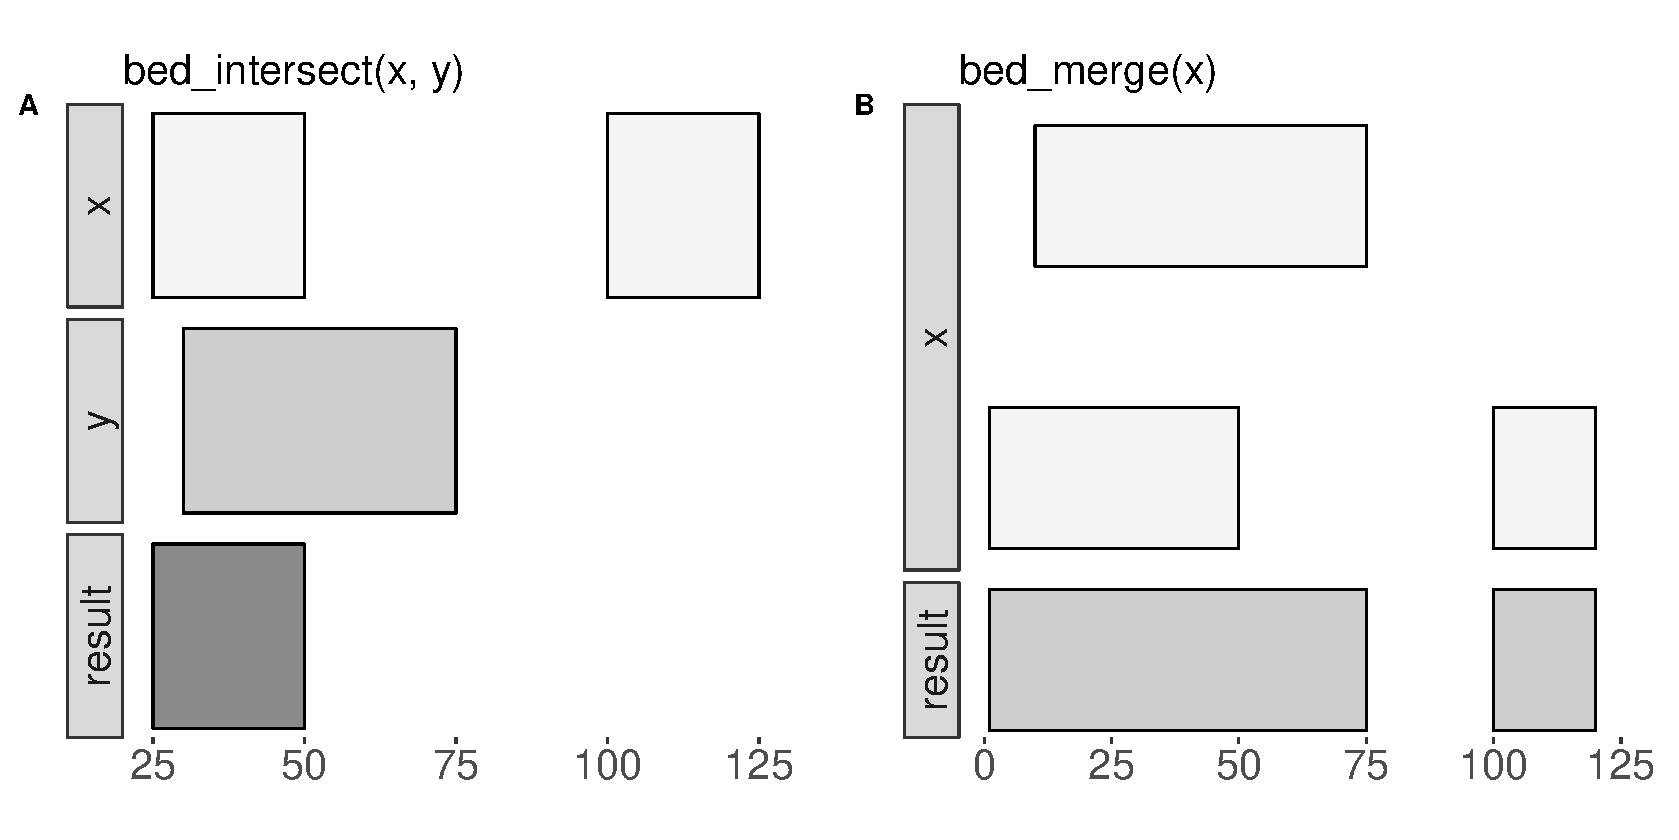
\includegraphics[width=1\textwidth]{figure1.pdf}
\caption{\label{fig:Figure 1}Visualizing interval operations in valr with \texttt{bed\_glyph()}.}
\end{figure}

%%%% Figure 2 %%%%

\begin{figure}[!htb]
\centering
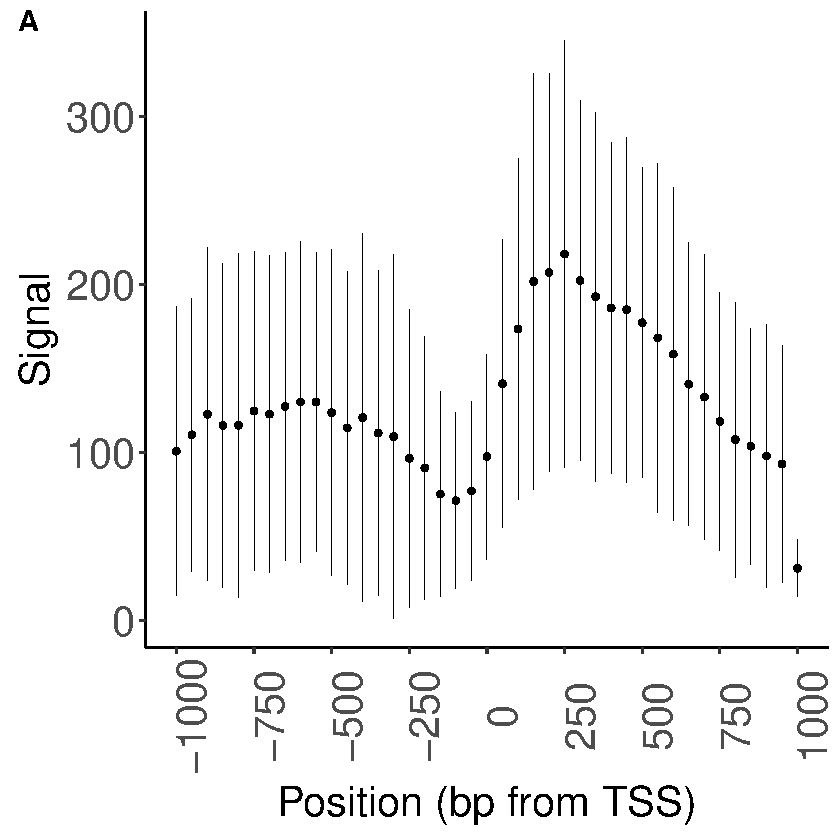
\includegraphics[width=0.5\textwidth]{figure2.pdf}
\caption{\label{fig:Figure 2}Meta-analysis of signals relative to genomic features with valr. \textnormal{(A) Summarized coverage of human H3K4Me3 Chip-Seq coverage across positive strand transcription start sites on chromosome 22. Data presented +/- SEM.}}
\end{figure}

%%%% Figure 3 %%%%
\begin{figure}[!htb]
\centering
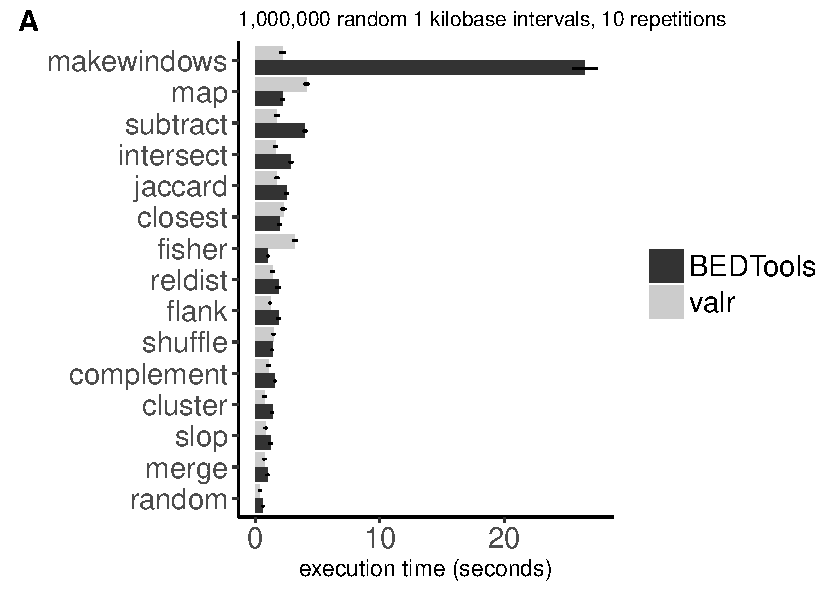
\includegraphics[width=1\textwidth]{figure3.pdf}
\caption{\label{fig:Figure 3} Performance of major valr functionality. \textnormal{(A)  Timings calculated by performing 10 repetitions of indicated functions on dataframes preloaded in R containing 1 million random 1 kilobase x/y intervals generated using \texttt{bed\_random()}. (B) Timings for executing functions in BEDTools or equivalent functions in valr using the same interval sets as in (A) written to files. All BEDTools function outputs were written to /dev/null/, and were timed using GNU \texttt{time}. Timings for valr functions in (B) include times for reading files using \texttt{read\_bed()} functions and were timed using the \texttt{microbenchmark} package.}}
\end{figure}


%%%% Table 1 %%%%

\begin{table}[h!]
\hrule \vspace{0.1cm}
\caption{\label{tab:tools} An overview of major functions available in valr.}
\centering
\begin{tabular}{lr}
 \bfseries \large Function Name & \bfseries  \large Purpose \\
  \hline
\bfseries Reading Data & \\
  read\_bed & Read BED files \\
  read\_bedgraph & Read bedGraph files \\
  read\_narrowpeak & Read narrowPeak files \\
  read\_broadpeak & Read broadPeak files \\
\bfseries Interval Transformation \\
  bed\_slop & Expand interval coordinates \\
  bed\_shift & Shift interval coordinates \\
  bed\_flank & Create flanking intervals \\
  bed\_merge & Merge overlapping intervals \\
  bed\_cluster & Identify (but not merge) overlapping intervals \\
  bed\_complement & Create intervals not covered by a query \\
\bfseries Interval Comparison & \\
  bed\_intersect & Report intersecting intervals from x and y tbls \\
  bed\_cluster & Cluster neighboring intervals \\
  bed\_map & Apply functions to selected columns for overlapping intervals \\
  bed\_subtract & Remove intervals based on overlaps \\
  bed\_window & Find overlapping intervals within a window \\
  bed\_closest & Find the closest intervals independent of overlaps \\
\bfseries Randomizing intervals & \\
  bed\_random & Generate random intervals from an input genome \\
  bed\_shuffle & Shuffle the coordinates of input intervals \\
\bfseries Interval statistics & \\
  bed\_fisher, bed\_projection & Calculate significance of overlaps between two sets of intervals \\
  bed\_reldist & Quantify relative distances between sets of intervals \\
  bed\_absdist & Quantify absolute distances between sets of intervals \\
  bed\_jaccard &Quantify extent of overlap between two sets of intervals \\
\bfseries Utilities &  \\
  bed\_glyph & Visualize the actions of valr functions \\
  bound\_intervals & Constrain intervals to a genome reference \\
  bed\_makewindows & Subdivide intervals \\
  bed12\_to\_exons & Convert BED12 to BED6 format \\
  interval\_spacing & Calculate spacing between intervals \\
  db\_ucsc, db\_ensembl & Access remote databases \\
  \end{tabular}
\end{table}

% See this guide for more information on BibTeX:
% http://libguides.mit.edu/content.php?pid=55482&sid=406343

% For more author guidance please see:
% https://f1000research.com/for-authors/article-guidelines/software-tool-articles


% When all authors are happy with the paper, use the
% ‘Submit to F1000RESEARCH' button from the menu above
% to submit directly to the open life science journal F1000Research.

% Please note that this template results in a draft pre-submission PDF document.
% Articles will be professionally typeset when accepted for publication.

% We hope you find the F1000Research Overleaf template useful,
% please let us know if yo\begin{Shaded}

\end{document}
